% Modified based on Xiaoming Sun's template
\documentclass{article}
\usepackage{amsmath,amsfonts,amsthm,amssymb}
\usepackage{setspace}
\usepackage{fancyhdr}
\usepackage{lastpage}
\usepackage{extramarks}
\usepackage{chngpage}
\usepackage{soul,color}
\usepackage{graphicx,float,wrapfig}
\usepackage{enumitem}
\usepackage{array} 
\newcommand{\Class}{Pattern Recognition and Machine Learning}

% Homework Specific Information. Change it to your own
\newcommand{\Title}{Homework 4}

% In case you need to adjust margins:
\topmargin=-0.45in      %
\evensidemargin=0in     %
\oddsidemargin=0in      %
\textwidth=6.5in        %
\textheight=9.0in       %
\headsep=0.25in         %

% Setup the header and footer
\pagestyle{fancy}                                                       %
\chead{\Title}  %
\rhead{\firstxmark}                                                     %
\lfoot{\lastxmark}                                                      %
\cfoot{}                                                                %
\rfoot{Page\ \thepage\ of\ \protect\pageref{LastPage}}                          %
\renewcommand\headrulewidth{0.4pt}                                      %
\renewcommand\footrulewidth{0.4pt}                                      %

%%%%%%%%%%%%%%%%%%%%%%%%%%%%%%%%%%%%%%%%%%%%%%%%%%%%%%%%%%%%%
% Some tools
\newcommand{\enterProblemHeader}[1]{\nobreak\extramarks{#1}{#1 continued on next page\ldots}\nobreak%
                                    \nobreak\extramarks{#1 (continued)}{#1 continued on next page\ldots}\nobreak}%
\newcommand{\exitProblemHeader}[1]{\nobreak\extramarks{#1 (continued)}{#1 continued on next page\ldots}\nobreak%
                                   \nobreak\extramarks{#1}{}\nobreak}%

\newcommand{\homeworkProblemName}{}%
\newcounter{homeworkProblemCounter}%
\newenvironment{homeworkProblem}[1][Problem \arabic{homeworkProblemCounter}]%
  {\stepcounter{homeworkProblemCounter}%
   \renewcommand{\homeworkProblemName}{#1}%
   \section*{\homeworkProblemName}%
   \enterProblemHeader{\homeworkProblemName}}%
  {\exitProblemHeader{\homeworkProblemName}}%

\newcommand{\homeworkSectionName}{}%
\newlength{\homeworkSectionLabelLength}{}%
\newenvironment{homeworkSection}[1]%
  {% We put this space here to make sure we're not connected to the above.

   \renewcommand{\homeworkSectionName}{#1}%
   \settowidth{\homeworkSectionLabelLength}{\homeworkSectionName}%
   \addtolength{\homeworkSectionLabelLength}{0.25in}%
   \changetext{}{-\homeworkSectionLabelLength}{}{}{}%
   \subsection*{\homeworkSectionName}%
   \enterProblemHeader{\homeworkProblemName\ [\homeworkSectionName]}}%
  {\enterProblemHeader{\homeworkProblemName}%

   % We put the blank space above in order to make sure this margin
   % change doesn't happen too soon.
   \changetext{}{+\homeworkSectionLabelLength}{}{}{}}%

\newcommand{\Answer}{\ \\\textbf{Answer:} }
\newcommand{\Acknowledgement}[1]{\ \\{\bf Acknowledgement:} #1}

%%%%%%%%%%%%%%%%%%%%%%%%%%%%%%%%%%%%%%%%%%%%%%%%%%%%%%%%%%%%%


%%%%%%%%%%%%%%%%%%%%%%%%%%%%%%%%%%%%%%%%%%%%%%%%%%%%%%%%%%%%%
% Make title
\title{\textmd{\bf \Class: \Title}}
  \date{\textbf{\today}}
\author{\textbf{Qingru Hu \quad 2020012996}}
%%%%%%%%%%%%%%%%%%%%%%%%%%%%%%%%%%%%%%%%%%%%%%%%%%%%%%%%%%%%%

\begin{document}
\begin{spacing}{1.1}
\maketitle \thispagestyle{empty}

%%%%%%%%%%%%%%%%%%%%%%%%%%%%%%%%%%%%%%%%%%%%%%%%%%%%%%%%%%%%%
% Begin edit from here

\begin{homeworkProblem}
% \Answer \\
\section*{(1)}
Use the linear property of expectation and expand the square of $E_{COM}$:
\begin{align*}
  E_{COM} = \frac{1}{M^2} (\sum_{m=1}^M \mathbb{E}_x[\epsilon(x)]^2 + 2 \sum_{m \neq l}^{M} \mathbb{E}_x[\epsilon_m(x) \epsilon_l(x)])
\end{align*}
All prediction model errors are zero-mean and uncorrelated, so the latter part disappears:
\begin{align*}
  E_{COM} = \frac{1}{M^2} \sum_{m=1}^M \mathbb{E}_x[\epsilon(x)]^2 
\end{align*}
We notice:
\begin{equation*}
  E_{AV} = \frac{1}{M} \sum_{m=1}^M \mathbb{E}_x[\epsilon(x)]^2 
\end{equation*}
Therefore:
\begin{equation*}
  E_{COM} = \frac{1}{M} E_{AV}
\end{equation*}

\end{homeworkProblem}

\begin{homeworkProblem}
\section*{(1)} See the decision\_tree.ipynb.
\section*{(2)}
\texttt{make\_split(variable, value, data, is\_numeric)}\\
\textbf{Input:}\\
\texttt{variable}, which is a str, the feature used to split the node;\\
\texttt{value}, which is either a number or str, the decision value for split, can be a quantitative value or a categorical feature;\\
\texttt{data}, which is a pandas dataframe, the subdataset at the split node. 
Each item of data represents whether the person is obese (1) or not (0).\\
\texttt{is\_numeric}, which is a bool, whether the split feature is numeric or categorical.\\
\textbf{Return:}\\
\texttt{data\_1}, which is a pandas dataframe, one child node dataset after split;\\
\texttt{data\_2}, which is a pandas dataframe, the other child node dataset after split.\\


\noindent\texttt{get\_best\_split(y, data)}\\
\textbf{Input:}\\
\texttt{y}, which is a str, the label, that is `obese' in this data; \\
\texttt{data}, which is a pandas datafram, the dataset at the node, constaining the features and labels;\\
\textbf{Return:}\\
\texttt{split\_variable}, which is a str, the feature that has the maximum IG at this node;\\
\texttt{split\_value}, the decision value for the split feature;\\
\texttt{split\_ig}, the value of the maximum IG;\\
\texttt{split\_numeric}, which is a bool, whether the split feature is numeric or categorical.

\section*{(3)}
\begin{figure}[htbp]
  \centering
  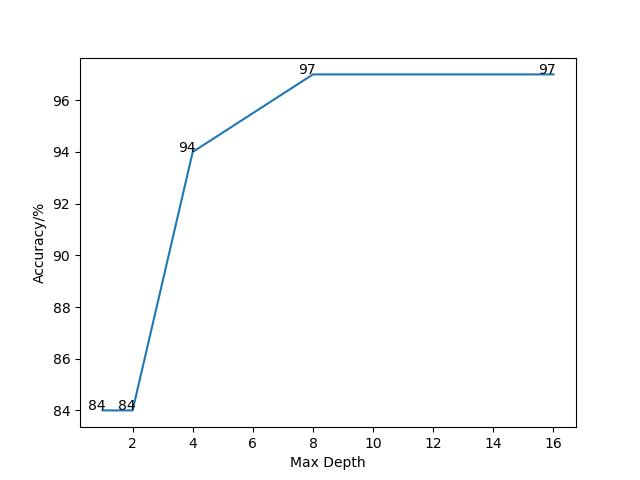
\includegraphics[width=10cm]{accu.png}
  \caption{The validation accuracy}
\end{figure}
The validation accuracy increases with the max depth of the decision from 1 to 8, 
but after 8 the validation accuracy remains the same when the max depth equals 8 and 16.
Since the validation doesn't decrease, overfitting does not occurred. 


The two other hyperparameters \texttt{min\_samples\_split} and \texttt{min\_information\_gain} have succesfully prevented the overfitting.
\end{homeworkProblem}


% \newpage
% \Acknowledgement{Thank Siying Yang 2020012981 for
% the discussion about Problem 2.3 and Problem 3.}

% End edit to here
%%%%%%%%%%%%%%%%%%%%%%%%%%%%%%%%%%%%%%%%%%%%%%%%%%%%%%%%%%%%%

\end{spacing}
\end{document}

%%%%%%%%%%%%%%%%%%%%%%%%%%%%%%%%%%%%%%%%%%%%%%%%%%%%%%%%%%%%%
